
\chapter{Module}
\label{cha:module}

Functions encapsulate pieces of code so that they can be reused throughout a program.
Modules collect sets of functions together so that they can be used by any number of programs.
Packages group sets of modules because their modules provide related functionality or because they depend on each other.



It is important to be aware of what the library can offer, since using predefined functionality makes programming much faster than creating everything from scratch.

Syntax for importing:
\begin{lstlisting}
import importable
import importable1, importable2, ..., importableN
import importable as preferred_name

from importable import object as preferred_name
from importable import object1, object2, ..., objectN
from importable import *

\end{lstlisting}



In the last syntex, the * means ``import everything that is not private'',
which in practical terms means
either every object in the module is imported except for those whose names begin with a leading underscore, or,
if the module has a global \argument{\_\_all\_\_} variable that holds a list of names, that all the objects named in the \argument{\_\_all\_\_} variable are imported.



How does Python know where to look for the modules and packages that are imported?

The built-in \argument{sys} module has a list called \argument{sys.path} that holds a list of the directories that consistutes the \keyword{Python path}.
The first directory is the directory that contains the program itself, even if the program was invoked from another directory.
If the \argument{PYTHONPATH} environment variable is set, the paths specified in it are the next ones in the list.
The final paths are those needed to access Python’s standard library --- these are set when Python is installed.

When we first import a module, if it isn’t built-in, Python looks for the module in each path listed in \argument{sys.path} in turn. 


Using byte-code compiled files leads to faster start-up times since the interpreter only has to load and run the code, rather than load, compile, (save if possible),and run the code;runtimes are not affected, though.
WhenPythonis installed, the standard library modules are usually byte-code compiled as part of the installation process.


\begin{figure}[!ht]
  \centering
  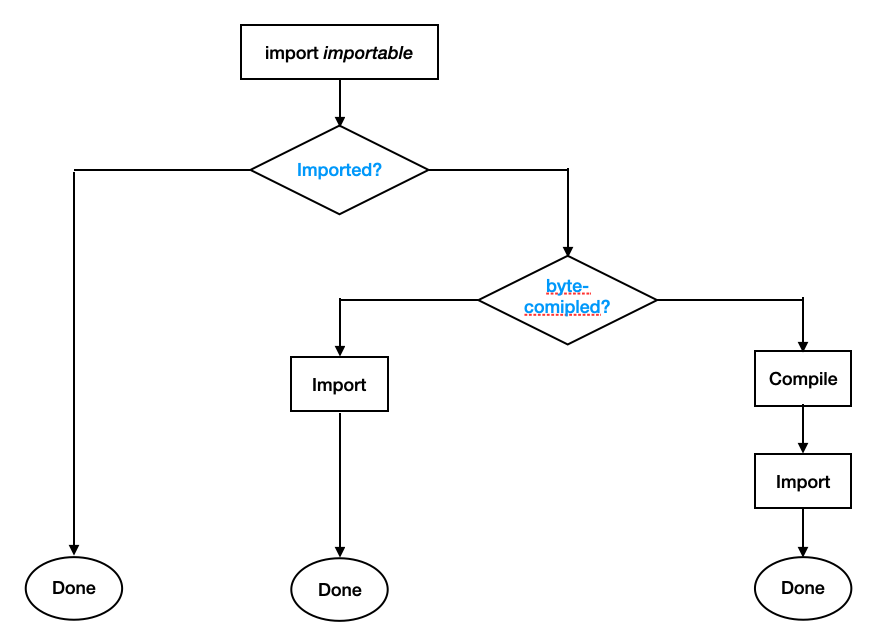
\includegraphics[width=0.8\textwidth]{images/import}
  \caption{Import process}
\end{figure}



\section{Package}
\label{cha:package}

A package is simply a directory that contains a set of modules and a file called \argument{\_\_init\_\_.py}.



In some situations it is convenient to load in all of a \keyword{package}’s modules using a single statement.
To do this we must edit the \keyword{package}’s \argument{\_\_init\_\_.py} file to contain a statement which specifies which modules we want loaded.
This statement must assign a list of module names to the special variable \argument{\_\_all\_\_}.



This syntax can also be applied to a module in which case all the functions, variables, and other object defined in the module (appart from those whose names begin with a leading underscore) will be imported.
If we want to control exactly what is imported, we can define an \argument{\_\_all\_\_} list in the module itself.

\section{Custom module}
\label{sec:custom-module}

You can define your own module.
If you want your module to be available to all your program, there are 3 approaches:
\begin{enumerate}
\item Put the module in the Python distribution's \argument{site-packages} subdirectory.
\item Create a directory for the custom modules and set the \argument{PYTHONPATH} environment variable to this directory
\item Put the module in the local site-packages subdirectory (\argument{/.local/lib/python3.9/site-packages})
\end{enumerate}


The second and third approaches have the advantage of keeping our own code separate from the official installation.


Doctesting is usually done by the following code:
\begin{lstlisting}
if __name__ == '__main__':
    import doctest

    doctest.testmod()
\end{lstlisting}


Whenever a module is imported Python creates a variable for the module called \argument{\_\_name\_\_} and store the modules name in this variable.
A modules name is simply the name of its \argument{.py} file but without the extension.

Whenever a \argument{.py} file is run Python creates a variable for the program called \argument{\_\_name\_\_} and sets it to the string \argument{\_\_main\_\_}.


%%% Local Variables:
%%% mode: latex
%%% TeX-master: "python"
%%% End:
